\scanpage{71}
\mspage{3}
sous-groupoïde induit sur une partie \uline{\unsure{finie}} \deleted{\illegible{1}} $I$ de $X_K$, on pourra trouver un nb fini de tels générateurs --- il suffit p.ex. de choisir un \deleted{\unsure{$x$}} $x_0\in I$, et choisir pour tt $x\in I\setminus x_0$ un chemin $l_x$ de $x_0$ \unsure{à} $x$, et de plus un syst. \inserted{fini} de générateurs $l_i$ de $\Pi_1(X,x_0)$.

Il apparaît que sous des conditions assez générales (p.ex. si $X$ est une variété alg. \unsure{anabélienne}) la connaissance de l'opération $u$ sur $\widehat{\Pi}_1(X_K,I)$ (\inserted{pour un} $u\in\Gamma$) \uline{suffit à} déterminer $u$ --- et la question se pose alors de voir comment la connaissance des invariants \inserted{disons} $g_{l_\alpha}(u)$ (pour un syst. générateur de flèches $l_\alpha$ de $\Pi_1(X,\unsure{I})$) permet de retrouver les invariants $g_l(u)$ pour d'autres \inserted{$K$-}schémas $Y\ldots$.
\margin{\figure{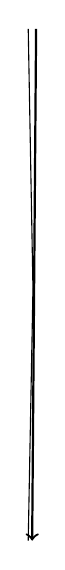
\begin{tikzpicture}[x=1mm,y=1mm]\draw (0,0)--(.6,32)--(0,65);\draw[->,line width=.8pt] (1,65)--(.5,0);\end{tikzpicture}}}

Quand il s'agit du $=$ schéma $X$, et qu'on s'intéresse \unsure{à} d'autres chemins $l:x\longrightarrow y$ $(x,y\in I)$ que les générateurs choisis $l_\alpha$, la formule donne en principe un moyen de reconstituer les $g_l(u)$ pour tout $l$, puisqu'il permet de retrouver les ${}^u l$, et que ${}^u l$ est multiplicatif en $l$. En termes des $g_l(u)$, \deleted{\unsure{$g_l(u)$}}, la formule de multiplicativité (6) s'écrit, pour une situation
\margin{\uline{NB} pour le moment, on ne regarde que les $x\in X_K$ qui sont dans $I$, le \unsure{syst} fini de \unsure{points} choisi.}
\diagram{\begin{tikzcd}[ampersand replacement=\&,column sep=large]
x\arrow[r,no head,"\unsure{l'|l}"] \& y\arrow[r,no head,"\unsure{l''|l'}"] \& z
\end{tikzcd}}
\[
(10)\qquad \unsure{g_{ll'}(\deleted{ll'}u)}=g_l(u)\cdot l\bigl(g_{l'}(u)\bigr)
\qquad\text{soit }g_u(ll')=g_u(l)\cdot l\bigl(g_u(l')\bigr)
\]
\margin{70}
